\chapter{Implementation}


\section{Environment}

The software developed in this thesis is completely realized using the Python programming language. This choice was made because OpenStack offers Python clients that connect to their API and the Elastic Media Manager is also programmed in Python.

PyCharm was selected as the Integrated Development Environment (IDE) to simplify the programming and testing lifecycles. The code is under revision control using Git and the repository that contains both the code for the CM and CM Agent consists of two main branches: master and develop. The develop branch holds the latest changes and upon successful testing those were merged back into master, which is always in a production-ready state.

\subsubsection{Project Structure}

The code is separated into two different projects in order to allow testing of the integration concurrently. The following graphic outlines the focus within the Elastic Media Manager (EMM), whilst the CM Agent is separated and has its own structure.

\begin{figure}[H]
\centering

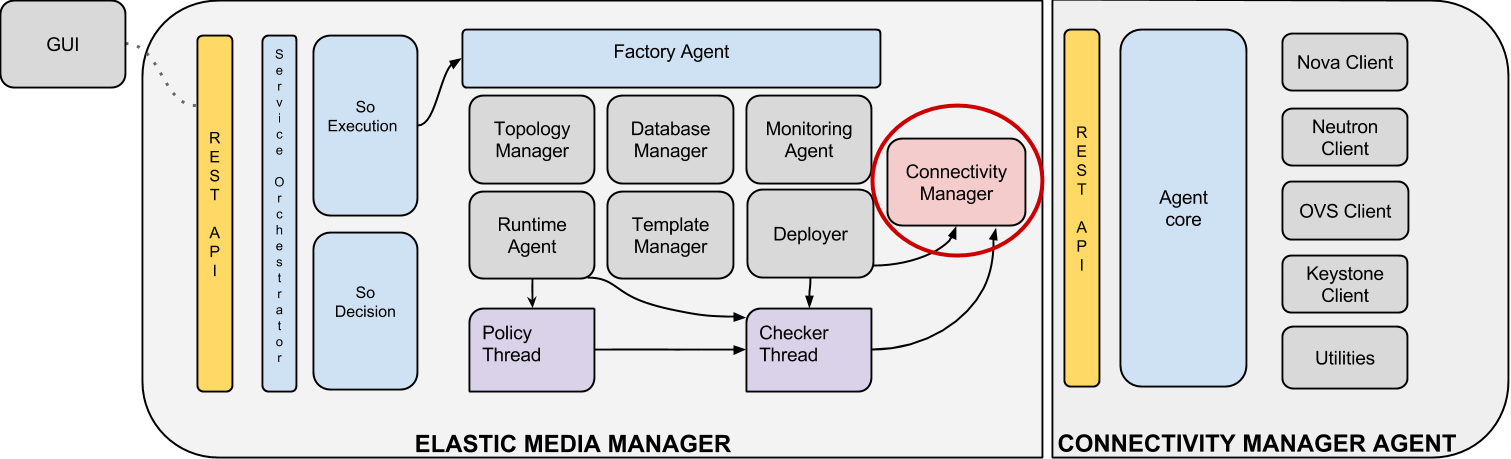
\includegraphics[width=0.9\textwidth]{images/implementation/cm_implementation_focus_overview}

\caption{Implementation focus}
\end{figure}

The structure for the CM is dictated by the already existing implementation of the EMM and the scope of this thesis includes solely its extension with a Connectivity Manager interface and service plus the needed changes in the other interfaces to make use of the methods within the CM.

The Connectivity Manager contains the ReST API, the Agent core, clients and other helper classes.

\subsubsection{Local OpenStack Test Environment}

In order to test the Connectivity Manager Agent and the use of its OpenStack API clients a test-bed was installed. This test-bed was set up using Vagrant, as it allows starting of the virtual machines from the command-line and can easily be provisioned and managed. In order to test the software across multiple compute nodes a setup with 2 VM's was installed.

For the installation of OpenStack, the devstack script was used, which takes care of not only the deployment of the different components but also their configuration. The configuration parameters are set in the 'local.conf' file. For the OpenStack cluster controller the following configuration was used:

\begin{lstlisting}[language=json]
[[local|localrc]]
ADMIN_PASSWORD=pass
DATABASE_PASSWORD=pass
RABBIT_PASSWORD=pass
SERVICE_PASSWORD=pass
SERVICE_TOKEN=a682f596-76f3-11e3-b3b2-e716f9080d50

HOST_IP=192.168.120.15
OVS_PHYSICAL_BRIDGE=br-ex
MULTI_HOST=1

# Enable Logging
LOGFILE=/opt/stack/logs/stack.sh.log
VERBOSE=True
OFFLINE=True
RECLONE=no
LOG_COLOR=True
SCREEN_LOGDIR=/opt/stack/logs

# Neutron
disable_service n-net
enable_service q-svc
enable_service q-agt
enable_service q-dhcp
enable_service q-l3
enable_service q-meta

# OpenStack API paths
MYSQL_HOST=192.168.120.15
RABBIT_HOST=192.168.120.15
GLANCE_HOSTPORT=192.168.120.15:9292
KEYSTONE_AUTH_HOST=192.168.120.15
KEYSTONE_SERVICE_HOST=192.168.120.15

IMAGE_URLS="$IMAGE_URLS,http://cloud-images.ubuntu.com/releases/trusty/
release/ubuntu-14.04-server-cloudimg-amd64-disk1.img"
\end{lstlisting}

The configuration file for the second node, which solely runs Nova, the Open vSwitch agent and the Rabbit MQ is identical except for its enabled services and host IP address:

\begin{lstlisting}[language=json]
HOST_IP=192.168.120.16
ENABLED_SERVICES=n-cpu,rabbit,neutron,q-agt,q-l3
\end{lstlisting}

During the implementation and testing phase the Connectivity Manager Agent was installed on the controller node while the EMM was executed from the local machine.

\section{Connectivity Manager - Components and Operations}

\subsubsection{Selection of Best-Performing Hypervisor}


\textbf{Step 1: Retrieve current host utilization from CM Agent}

In order to decide on the placement, the Connectivity Manager firstly needs to retrieve the host information from the Agent. It then sums up the different resource utilizations: amount of servers currently running on it, the total amount of used RAM \& vCPUs.
\begin{figure}[H]
\centering

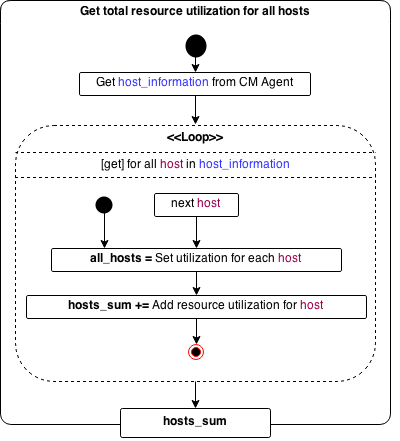
\includegraphics[width=0.4\textwidth]{images/implementation/cm_get_host_utilization}

\caption{Check resource utilization of hosts}
\end{figure}

The amount of resources that are required in total to deploy the topology on the tenant needs to be calculated by adding up the amount of resources that are needed for each Unit. This can easily be done by checking its flavor.

\begin{figure}[H]
\centering

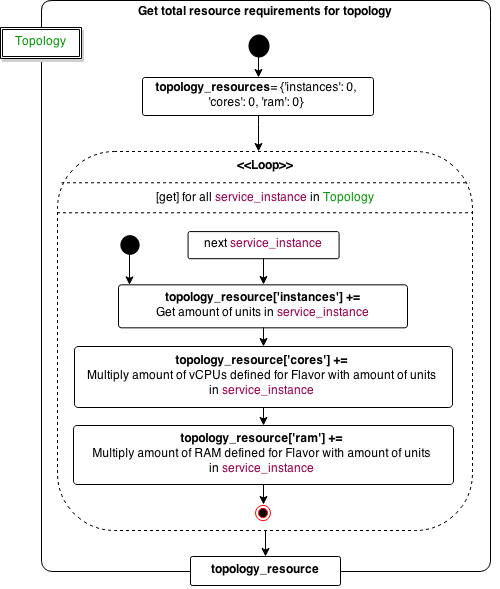
\includegraphics[width=0.5\textwidth]{images/implementation/cm_get_topology_requirements}

\caption{Get total amount of required resources for topology}
\end{figure}

\textbf{Step 2: Check if Topology is within the limitations of the Quota and currently available resources on the tenants hosts.}

In the second step it is checked if the topology is feasible for deployment. This decision is made by first comparing the values from Step 1 to the available Quota values (amount of VMs, RAM, and vCPUs required for the sum of all servers) and secondly finding out if the required resources are less or equal to the currently not utilized resources in the tenants infrastructure.

\begin{figure}[H]
\centering

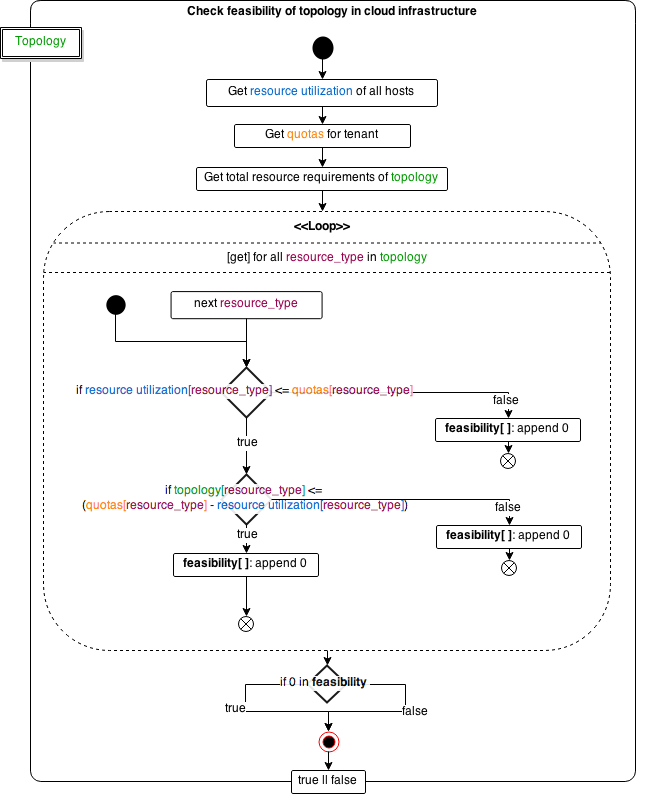
\includegraphics[width=0.6\textwidth]{images/implementation/cm_feasibility_check}

\caption{Deployment feasibility check}
\end{figure}

These comparisons need to be made, in order to conform to the requirement of not over-committing any resources.


\textbf{Step 3: Check whether the Topology can be deployed on a single host.}

The next step checks if the total amount of topology resources from Step 1 can be deployed on a single host. If there are multiple hosts that have enough capacity available, the first one within the list is returned by this method.

\begin{figure}[H]
\centering

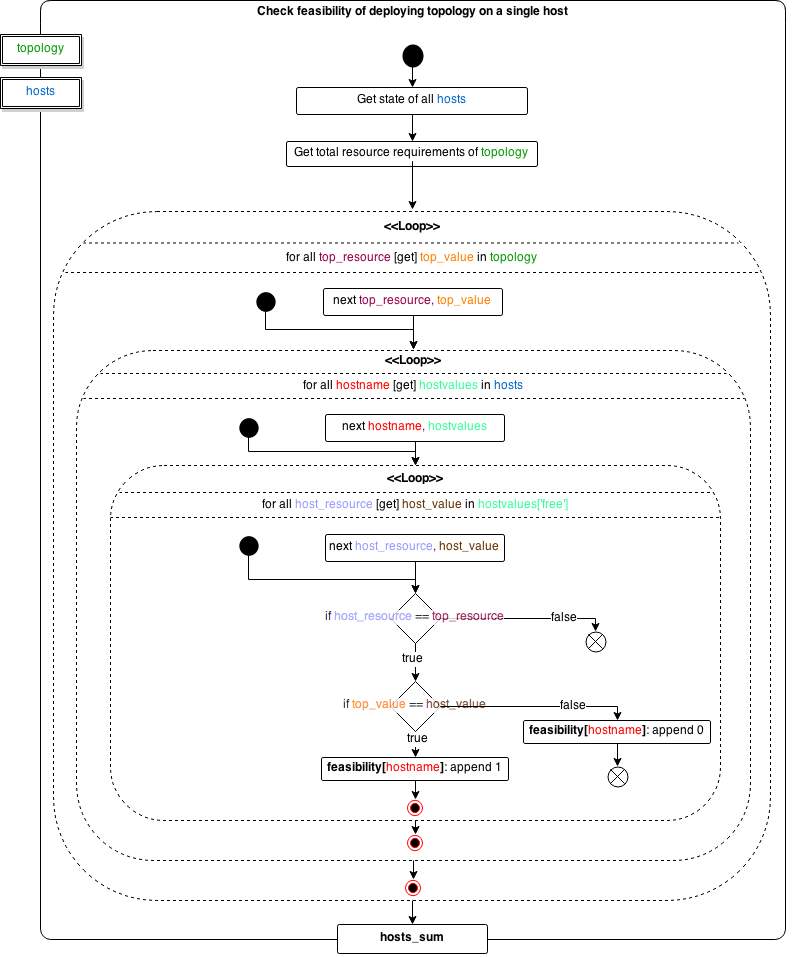
\includegraphics[width=0.7\textwidth]{images/implementation/cm_single_host_check}

\caption{Single host deployment check}
\end{figure}


\textbf{Step 4: Set selected host as availability zone for each Unit.}

Lastly the chosen host needs to be set in the topology, so it can be returned to Heat for continuing with the deployment process. The syntax for a Unit's availability zone needs the 'nova' suffix, so this string needs to be added in front of the host name.

\begin{figure}[H]
\centering

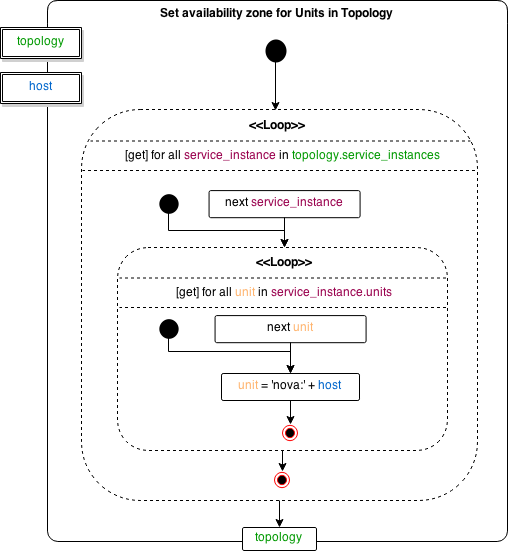
\includegraphics[width=0.5\textwidth]{images/implementation/cm_set_az_topology}

\caption{Set AZ per Unit}
\end{figure}

\subsubsection{Enabling QoS for servers}

The rates for the QoS classes can be set in the configuration of the EMM.
The default location is \textit{/etc/nubomedia/emm.properties} and it contains the following default rates:
\begin{lstlisting}[language=commands]
# CONNECTIVITY MANAGER PROPS & QOS RATES (IN BIT/S)
cm_agent_ip=192.168.41.45
# GOLD = 100MBIT/S - 10GBIT/S
gold_min=100000000
gold_max=10000000000
# WHOLESALE = 100MBIT/S - 1GBIT/S
wholesale_min=100000000
wholesale_max=1000000000
\end{lstlisting}

For setting QoS for all Units within a Service Instance, the following workflow is passed through:

\begin{figure}[H]
\centering

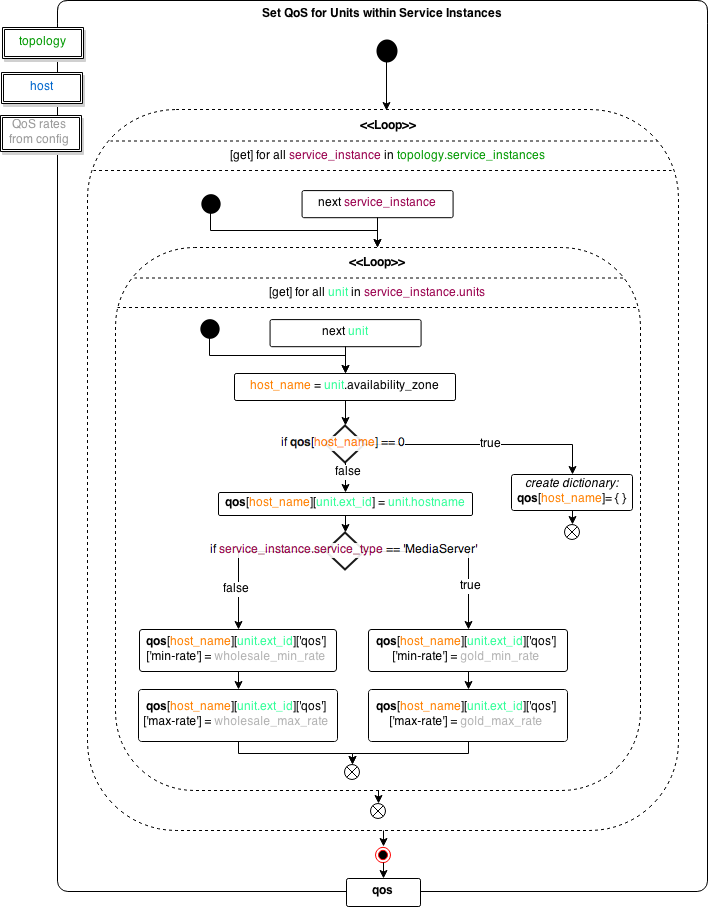
\includegraphics[width=0.6\textwidth]{images/implementation/cm_set_qos.png}

\caption{Method for setting QoS for all Units}
\end{figure}

The dictionary that this method returns is then converted to the JSON format and sent to the Connectivity Manager Agent by performing a HTTP POST to the \textit{/qoses} path of the IP address that is set for the \textit{cm\_agent\_ip} property in the configuration file.

\section{Connectivity Manager Agent - Components and Operations}

The two major operations that the Connectivity Manager needs to perform in order to provide the required services to this project is retrieving the resource status of the data center and setting QoS for the servers ports.

For using the OVS Client it needs to access the OVSDB that is located on each host. In order to allow that, the following command needs to be executed on them once:
\begin{lstlisting}[language=commands]
$ sudo ovs-vsctl set-manager ptcp:6640
\end{lstlisting}

This enables remote administration through a passive TCP connection using the local IP address and port 6640. 

\subsection{Get list of all hosts and their utilization state}

The following figure displays the way in which the CM Agent creates a dictionary containing the list of all hosts within the selected tenant. It contains information such as the amount of already running virtual machines, the amount of allocated RAM in MB and the number of vCPUs in use. For each of the virtual machines it shows their ID, name, and further resource information that is later needed for setting QoS. In case the VM already has a QoS assurance attached to its port, the corresponding minimal and maximal rates are shown.

\begin{figure}[H]
\centering

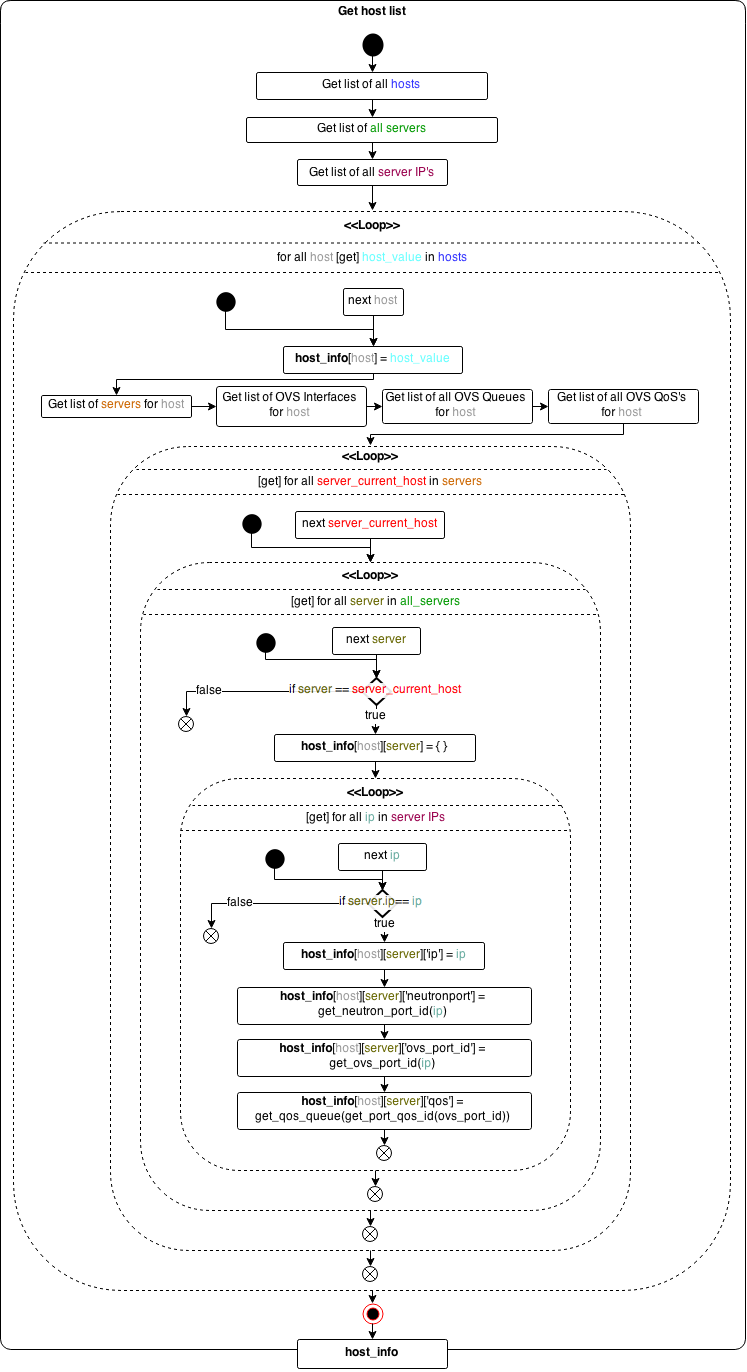
\includegraphics[width=0.65\textwidth]{images/implementation/cma_host_list}

\caption{Get list of hosts}
\end{figure}

In order to identify the rates that might have already been attached to a VM's port, a few steps need to be taken. With the server's IP address the Neutron Port ID can be retrieved. This Neutron Port ID has a Port ID within Open vSwitch that can be retrieved from the OVSDB. 

\begin{figure}[H]
\centering

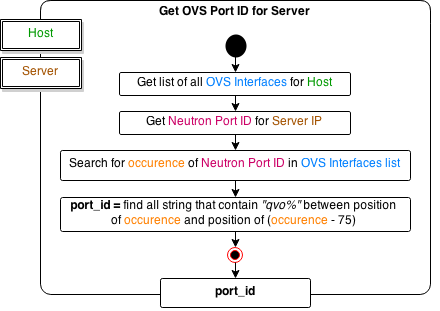
\includegraphics[width=0.5\textwidth]{images/implementation/cma_get_ovs_port_server}

\caption{Get OVS Port ID for server}
\end{figure}

Each Port contains a field for QoS, which holds its QoS ID. This ID can then be filtered from the Queue table.

\begin{figure}[H]
\centering

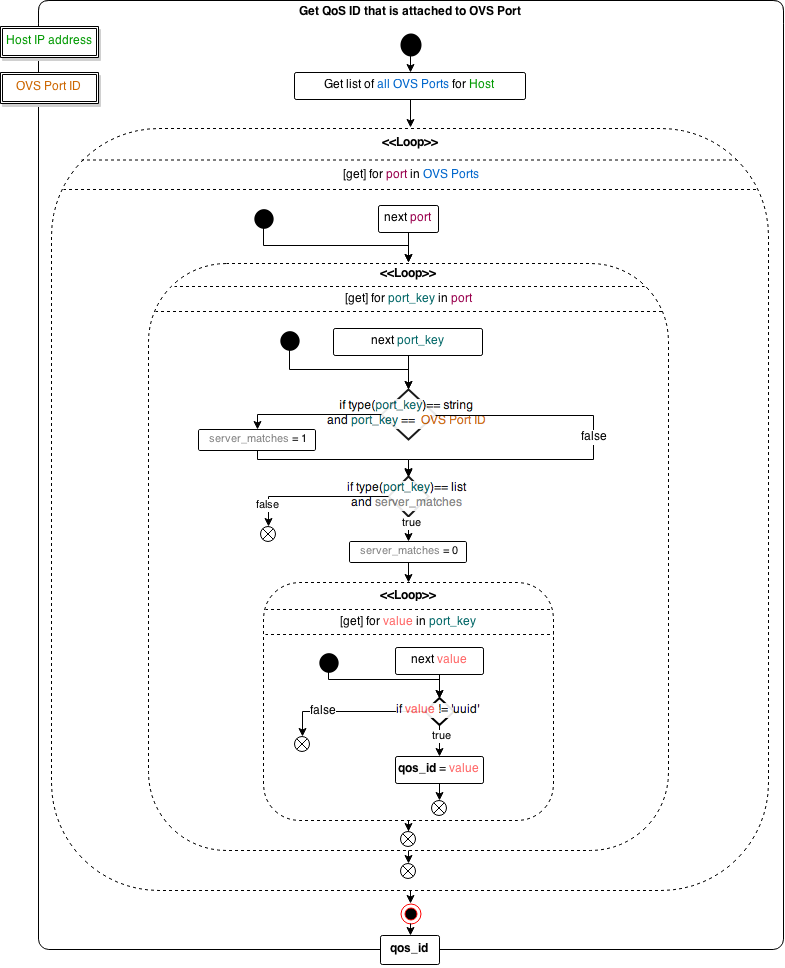
\includegraphics[width=0.7\textwidth]{images/implementation/cma_get_qos_id_for_ovs_port}

\caption{Get QoS ID for OVS Port}
\end{figure}

The QoS ID has a Queue attached to it, wherein the set minimum and maximum bandwidth rates are specified.

\begin{figure}[H]
\centering

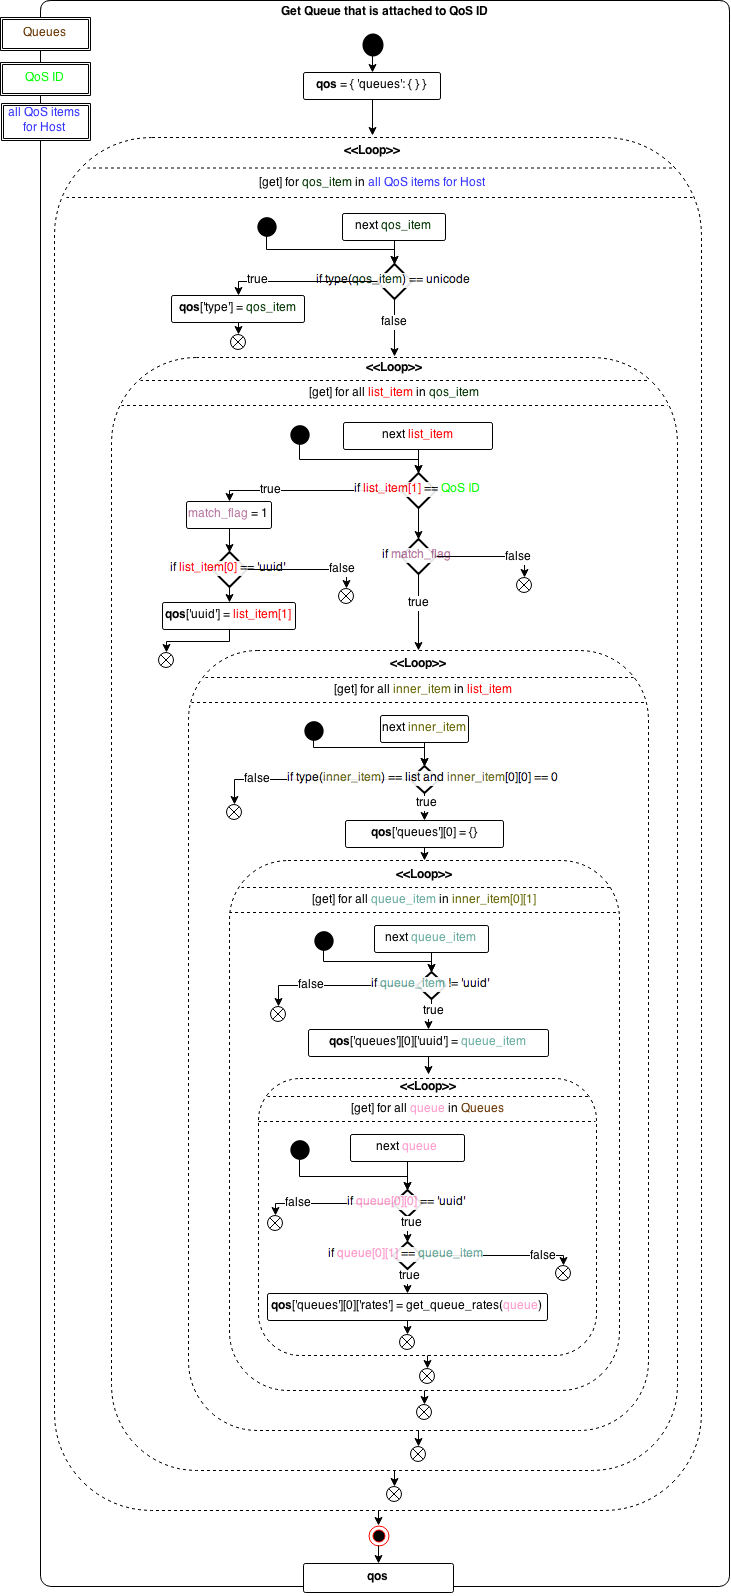
\includegraphics[width=0.7\textwidth]{images/implementation/cma_get_queue_rates_for_qos}

\caption{Get Queue rates for a QoS ID}
\end{figure}


\subsection{Set QoS rates for all servers}

In order to set the bandwidth rates for the servers this method first retrieves the list of all hosts that was mentioned in the previous figure and description. When the \textit{Set QoS} method is called through a request to the API the method body from the HTTP POST is passed onto it. This dictionary contains all QoS rates that need to be set for each server. 


\begin{figure}[H]
\centering

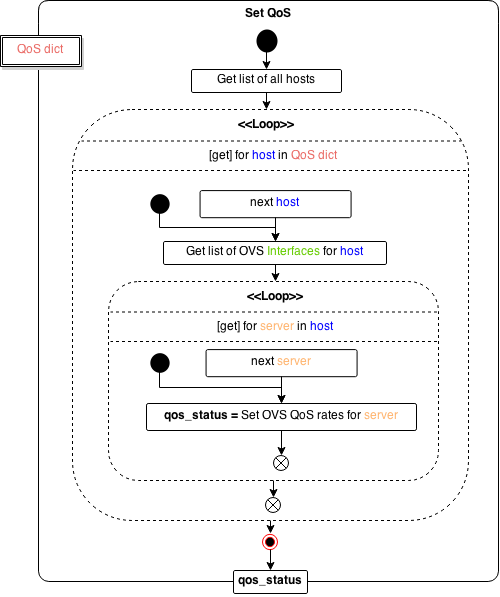
\includegraphics[width=0.5\textwidth]{images/implementation/cma_set_qos}

\caption{Set requested QoS rates for all servers}
\end{figure}

The method that is called from within the above figure for setting QoS for a single server performs the following activities:

\begin{figure}[H]
\centering

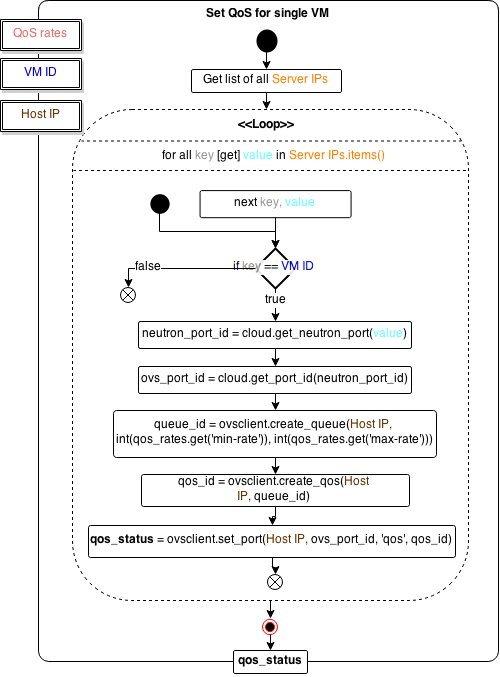
\includegraphics[width=0.4\textwidth]{images/implementation/cma_set_qos_single_server}

\caption{Set QoS rates for a single server}
\end{figure}

\subsection{API}

The API was implemented using Bottle. It is a fast, simple and lightweight WSGI micro web-framework \cite{bottle-docs}. Therein three routes were defined:
\begin{lstlisting}[language=json]
# Welcome Screen
self._app.route('/', method="GET", callback=self._welcome)
# Host method
self._app.route('/hosts', method="GET", callback=self._hosts_list)
# QoS method
self._app.route('/qoses', method=["POST", "OPTIONS"], callback=self._qoses_set)
\end{lstlisting}

The first route contains a welcome message and can be used to check if the WSGI app is currently running.
The /hosts route calls the list\_hosts() method in the Agent when a HTTP GET is received.
When the /qoses route is called with the QoS parameters in its HTTP body it calls the set\_qos() method in the Agent class.

The server uses the localhost IP address and is served and listens on port 8091. It is important that this IP address is whitelisted in case a firewall exists. In the case of using a Vagrant box the port needed to be forwarded to the local machine.

\section{Tests}

For testing the components of the Connectivity Manager Agent the code was synchronized to a local testbed with two virtual machines, one of which acted as the control node and the other just as a compute node. 

\begin{figure}[H]
\centering

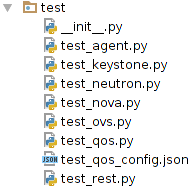
\includegraphics[width=0.17\textwidth]{images/implementation/cma_tests.png}

\caption{Connectivity Manager Agent: Test package}
\end{figure}

These functional tests contain the following methods of the main components:
\begin{itemize}
\item Agent: instantiates the Agent class and tests listing the information about all hosts
\item Keystone: tests retrieving the token and endpoint
\item Neutron: lists all ports and shows the Neutron Port ID for a selected IP address
\item Nova: retrieves all hosts and their servers
\item OVS: tests the main functionalities that are used within this work: listing all interfaces, ports, queues, qos's and creating a new queue and qos that are then attached to a OVS port
\item QoS: takes the parameters set in the \textit{test\_qos\_config.json} file as an input and posts it to the API in order to try and set QoS on the defined server ports
\item ReST: tests retrieving the list of all hosts through the API
\end{itemize}

The tests for the Connectivity Manager are part of the testing packages of the Elastic Media Manager, because that is the only way they are called. The \textit{test\_deploy.py} was used for checking if the integration works successfully.  It uses a predefined topology from a local file. The following minimized configuration was used during the tests:
\begin{lstlisting}[language=json]
{
    "name":"local_nm_template_minified",
    "service_instances": [
        {
            "name":"Controller",
            "service_type":"Controller"
        },
        {
            "name":"Broker",
            "service_type":"Broker"
        }
    ]
}
\end{lstlisting}

To find out more about the parameters that each of the service\_types corresponds to, please check the \textit{Topology Definition} % % LINK TO SECTION % %
in the Evaluation section.